\documentclass[11pt,a4paper]{article}
\usepackage[utf8]{inputenc}
\usepackage[french]{babel}
\usepackage[T1]{fontenc}
\usepackage{amsmath}
\usepackage{amsthm}
\theoremstyle{definition}
\newtheorem*{definition}{Definition}
\theoremstyle{remark}
\newtheorem*{remark}{Remark}
\setcounter{secnumdepth}{3}
\usepackage{float}
\usepackage{amsfonts}
\usepackage{amssymb}
\usepackage{graphicx}
\usepackage{setspace}
\usepackage{gensymb} %Pour le degré
\usepackage{titlesec} %Pour le 3ème niveau de titres
\usepackage{fancyvrb} %Pour le Verbatim
\usepackage{alltt} %Environnement pseudo code
\usepackage{listings}% http://ctan.org/pkg/listings
\usepackage{listingsutf8}
\usepackage{geometry}
\lstset{
  basicstyle=\ttfamily,
  mathescape,
	literate={é}{{\'e}}1
           {è}{{\''e}}1
}
\lstinputlisting[inputencoding=utf8/latin1]

\newcommand{\reporttitle}{Rapport final}
\newcommand{\reportauthor}{Clément \textsc{Tamines} Jérémy \textsc{Gheysen}}
\newcommand{\reportsubject}{Projet de Structures de Données II}
\newcommand{\HRule}{\rule{\linewidth}{0.5mm}}
\renewcommand{\ttdefault}{txtt} %Pour le gras environnement pseudo-code

\setcounter{secnumdepth}{4}
\titleformat{\paragraph}
{\normalfont\normalsize\bfseries}{\theparagraph}{1em}{}
\titlespacing*{\paragraph}
{0pt}{3.25ex plus 1ex minus .2ex}{1.5ex plus .2ex}

\makeindex
\begin{document}
%TODO : Ajouter à la table des matières les paragraphes

%Page de garde
\begin{titlepage}
\begin{center}
\begin{minipage}[t]{0.48\textwidth}
  \begin{flushleft}
     
\includegraphics[width=42mm]{UMONS+txt.pdf} \\[0.5cm]
  \end{flushleft}
\end{minipage}
\begin{minipage}[t]{0.48\textwidth}
  \begin{flushright}
    
\includegraphics [width=42mm]{UMONS_FS.pdf} \\[0.5cm]
  \end{flushright}
\end{minipage} \\[1.5cm]

\vspace{1.5cm}
\textsc{\Large \reportsubject}\\[0.5cm]
\HRule \\[0.4cm]
{\huge \bfseries \reporttitle}\\[0.4cm]
\HRule \\[1.5cm]

\begin{minipage}[t]{0.3\textwidth}
  \begin{flushleft} \large
    \emph{Auteurs :}\\
    \reportauthor
  \end{flushleft}
\end{minipage}
\begin{minipage}[t]{0.6\textwidth}
  \begin{flushright} \large
    \emph{Professeur :} \\
    V. \textsc{Bruyère} \\
     \emph{Assistant :} \\
    G. \textsc{Devillez}
  \end{flushright}
\end{minipage}
\vfill
{\large 15 avril 2016}

\end{center}
\end{titlepage}

\tableofcontents
\newpage

\section*{Introduction}
\addcontentsline{toc}{section}{Introduction}
Ce projet consiste en l'implémentation d'un outil permettant, à partir d'un point de vue et d'une scène composée de segments colorés placés dans un repère orthonormé, d'afficher la scène telle que perçue par ce point de vue. Ce point de vue pourra être placé dans le repère par l'utilisateur.\\

Pour réaliser cet affichage, nous utiliserons l'algorithme du peintre tel que décrit dans le Chapitre 12 du livre \textit{Computational Geometry}. Cet algorithme s'applique sur des arbres qui stockent l'ensemble de segments qui compose la scène et qui permettent de trouver un ordre d'affichage correct pour un point de vue quelconque. Ces arbres sont appelés arbres BSP (\emph{Binary Spaces Partition}) et seront construit via différentes techniques à partir d'une liste de segments définis par leurs sommets et leur couleur. Nous présenterons dans ce rapport la technique \textit{in-order}, sa variante \textit{random} et le principe des \textit{free-splits}.\\

Ce rapport a pour but de décrire les différentes techniques et algorithmes utilisés lors de la construction des arbres BSP et de la visualisation de la scène à l'aide de l'algorithme du peintre. Nous analyserons également la complexité et la performance de ces algorithmes.

\newpage

\section{Arbres BSP}

\subsection{Principe et définitions}
Un arbre BSP (\emph{Binary Space Partition}) est un arbre binaire permettant de stocker de manière efficace un ensemble d'objets (dans notre cas des segments) situés dans un plan. Rappelons tout de même qu'un arbre binaire est un arbre tel que tout nœud possède au plus deux fils.\\

Les arbres BSP étudiés ici consistent en une séparation binaire du plan, s'effectuant de manière récursive. Ce processus sépare donc le plan en plusieurs régions, chacune d'entre elles contenant des segments. La séparation du plan se termine lorsque chaque région ne contient plus qu'un segment.\\

Chaque nœud possède un ensemble de segments $i$ dans un hyperplan et définit une nouvelle séparation binaire de ce dernier, cela sur base d'une droite de séparation $s$ (choisie selon une technique définie au préalable et dans laquelle sont contenus un ou plusieurs segments), et sépare ainsi le plan en deux sous-espaces $s^+$ et $s^-$ contenant chacun une partie des segments de $i$ non contenus dans la droite de séparation (les segments contenus dans $s$ étant les segments importants à stocker dans le nœud). Cette méthode de séparation est alors appelée récursivement sur chacun des deux sous-espaces nouvellement créés qui seront stockés dans les deux fils de ce nœud. La droite $s$ utilisée pour séparer le plan peut néanmoins couper des segments en deux, résultant alors dans la création de deux nouveaux segments qui seront contenus dans $s^+$ et $s^-$. Remarquons qu'avec la manière avec laquelle nous définissons chaque nouveau nœud, les feuilles de l'arbre seront des nœuds possédant une droite de séparation $s$ dans laquelle seront contenus un ou plusieurs segments. Ces feuilles ne pourront donc pas avoir de fils, puisqu'elles ne posséderont aucun segments dans $s^+$ et $s^-$.\\

\theoremstyle{Definition}
\begin{definition}{Arbre BSP}\\
\textit{-Cas de base :} Un arbre BSP vide est un arbre BSP\\
\textit{-Cas général :} Un arbre BSP est un composé d'un nœud contenant une droite de séparation $s$, une liste chaînée de segments contenus dans cette droite et une liste chaînée $i$ de segments dont ont doit déterminer si ils sont dans $s^+$ ou $s^-$. Il possède aussi deux fils qui sont eux-même des arbres BSP et qui auront pour liste de segments $i$ les segments contenus dans $s^+$ ou $s^-$.
\end{definition}

\theoremstyle{Definition}
\begin{definition}{Taille d'un arbre BSP}\\
La taille d'un arbre BSP est calculée en fonction du nombre total de segments que celui-ci contient. Cette valeur est donc la somme, pour chaque nœud de l'arbre, du nombre de segments contenus dans la droite de séparation $s$ de ce nœud. Ce calcul de taille prend donc en compte le fait que des segments peuvent être coupés en plusieurs fragments.\\
\end{definition}

Les méthodes de construction des arbres seront présentées plus loin dans ce rapport.

\subsection{Structures de données}
Afin de représenter les différents éléments du problème, nous avons créé plusieurs objets et structures de données.

\subsubsection{Segment}
La classe Segment permet, comme son nom l'indique, de représenter un segment dans le plan. Celui-ci est définit à partir de deux extrémités $(x_1,y_1)$, $(x_2,y_2)$ et d'une couleur. Un segment possède également trois autres propriétés (\emph{intersected, isFreeSplit, intersection}), nécessaires à l'implémentation de l'heuristique des free-splits. Nous nous attarderons sur ces éléments plus tard. \\

Ci-dessous sont présentées les méthodes sur ces segments les plus importantes pour la suite des calculs :\\

\begin{itemize}
\item \emph{computeLine} : Calcule l'équation de la droite qui contient le segment sous la forme $ax + by + c = 0$ et la stocke dans un tableau de dimension trois contenant ses coefficients $a,b,c$;
\item \emph{getSide} : Remplace les coordonnées $x$ et $y$ données en paramètres dans la droite également donnée en paramètre et retourne le résultat (0 si le point est sur la droite). Ceci nous permet de savoir de quel coté de la droite le point se trouve;
\item \emph{computePosition} : Retourne la position relative du segment par rapport à la droite donnée en paramètre. Remarquons que pour cette méthode certaines conventions ont été prises. En effet, si il y a une intersection entre le segment et la droite, cette dernière est retournée dans un tableau à deux dimensions représentant un point. Sinon si le segment est à gauche de la droite, NaN est retourné, si il est à droite, Infinity qui est retourné. Notons également que si nous nous trouvons dans le cas où il y a intersection au niveau d'un sommet du segment, par facilité d'implémentation nous retournerons que celui-ci est à gauche ou à droite en ignorant l'intersection.
\end{itemize}

\subsubsection{Nœud BSP} 
La classe BSPNode permet de représenter un nœud d'un arbre BSP définit de manière récursive. Un nœud possède une droite de séparation $s$ stockée sous la forme d'un tableau de dimension trois contenant ses coefficients $a,b,c$ de l'équation $ax + by + c = 0$ de la droite. Bien évidemment, chaque nœud contient aussi une référence vers son fils gauche $leftSon$ et son fils droit $rightSon$. 
Le nœud contient aussi deux listes chaînées de segments :\\

\begin{itemize}
\item \emph{segmentsInLine} : stocke les segments contenus dans la droite $s$;
\item \emph{segmentsInHyperplane} : stocke les segments contenus dans la région du plan obtenue en suivant les séparations successives effectuée par chaque nœud à partir de la racine de l'arbre;
\end{itemize}

\subsubsection{Listes chaînées}

Nous avons fait le choix d'utiliser les listes chaînées pour stocker des segments.\\
L'avantage de ces structures de données est la récupération du premier élément et sa suppression en O(1). En effet, une référence au début de la liste étant toujours gardée, il est très peu coûteux d'y accéder et de le supprimer. Étant donné que les segments sont traités dans l'ordre de la liste dans le but de créer une ligne de séparation $s$, il est intéressant de pouvoir facilement accéder au premier segment.\\
Dans un second temps, il est utile de remarquer que l'ajout d'un segment dans une liste chaînée se fait aussi en O(1) via l'utilisation d'une référence vers le dernier élément de la liste. Ceci est très utile vu que des segments sont ajoutés à des listes chaînées constamment (notamment les fragments ajoutés à ces listes suite à la coupure d'un segment).

\subsection{Construction}

\subsubsection{Heuristique "in-order"}

\paragraph{Méthode}

Cette heuristique est très intuitive et met simplement en pratique le principe des arbres BSP. Étudions son fonctionnement à l'aide de l'exemple représenté à la Figure \ref{scene_inordre}. 

\begin{figure}[H]
\centering
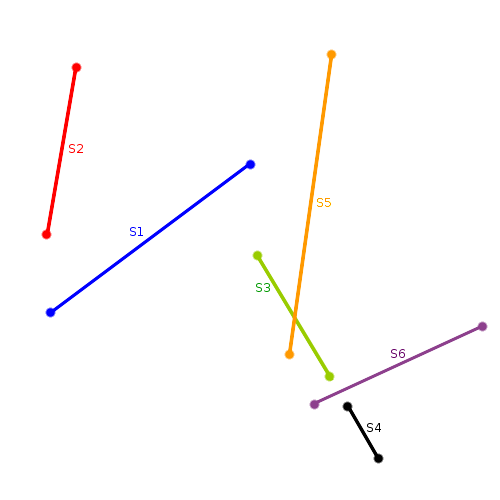
\includegraphics[scale=0.5]{bsp_ex_1.png}
\caption{Scène de segments}
\label{scene_inordre}
\end{figure}

Nous pouvons remarquer que cette scène contient 6 segments distincts, dont deux (les segments S3 et S4) se situant sur une même droite. Nous avons également des segments qui s'intersectent, ce qui va inexorablement mener à la création de nouveaux segments. Nous allons maintenant appliquer l'heuristique "in-ordre" sur l'exemple de la figure \ref{scene_inordre} et en expliquer le fonctionnement. L'arbre BSP correspondant est construit à la Figure \ref{bsp_tree}. \\

Cette heuristique travaille avec la liste des segments telle qu'elle a été fournie par l'utilisateur, c'est à dire que la création de l'arbre se fait dans l'ordre par lequel les segments ont été définis. Dans notre exemple, la liste de segment initiale $i$ contient les segments dans l'ordre suivant : $\{S1,S2,S3,S4,S5,S6\}$ \\

Nous commençons donc par une division du plan à l'aide de la droite qui contient S1 que nous noterons $s_1$. Nous remarquons d'ores et déjà que S5 est coupé en deux segments S5A et S5B. Nous obtenons donc maintenant deux sous-ensembles de $i$, qui sont les segments contenus dans les régions $s_1^+$ et $s_1^-$: \\
$$s_1^+ \quad contient\quad \{S2, S5A\}$$
$$s_1^- \quad contient\quad \{S3,S4,S5B,S6\}$$

\begin{figure}[H]
\centering
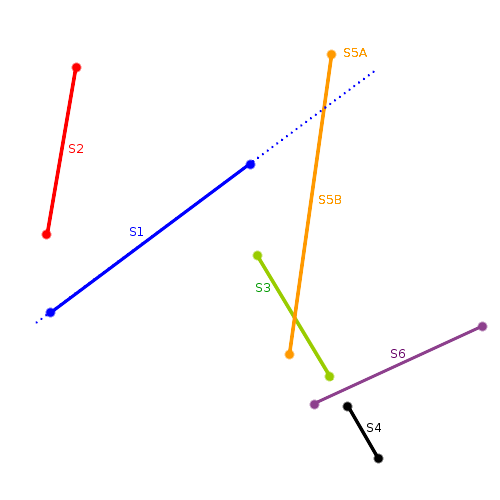
\includegraphics[scale=0.6]{bsp_ex_2.png}
\caption{Application de l'heuristique sur le nœud dont la droite est construite via $S1$}
\label{bsp_inordre}
\end{figure}\\
\newpage

Le nœud va donc contenir le segment $S1$ dans la liste de segments contenus dans sa droite de séparation $s_1$. L'algorithme va être appelé récursivement sur deux nœuds dont les listes de segments sont celles définie précédemment. Là encore, le premier segment de chacune de ces listes sera utilisé pour construire la droite de séparation.\\

La première liste contiendra ainsi les segments $\{S2, S5A\}$. Le segment $S2$ sera utilisé pour créer la ligne de séparation $s_2$, le nœud contiendra dans sa liste de segments contenus dans la droite le segment $S2$. Nous remarquons alors que suite à la séparation du plan par la droite $s_2$, $s_2^+$ et $s_2^-$ contiennent les segments suivants:\\
$$s_2^+ \quad \text{ne contient pas de segments}$$
$$s_2^- \quad contient\quad \{S5A\}$$
\\
Le nœud actuel ne possédera alors pas de fils droit et aura un fils gauche qui sera une feuille (puisqu'il contiendra uniquement $S5A$).\\

\begin{figure}[H]
\centering
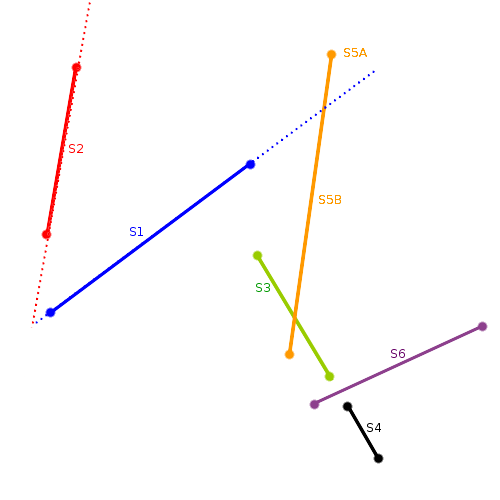
\includegraphics[scale=0.6]{bsp_ex_4.png}
\caption{Application de l'heuristique sur le nœud dont la droite est construite via $S2$}
\label{bsp_ex_4}
\end{figure}
\newpage

La deuxième liste contiendra ainsi les segments $\{S3,S4,S5B,S6\}$. Le segment $S3$ sera utilisé pour créer la ligne de séparation $s_3$, nous remarquons que le segment $S4$ est lui aussi compris dans cette droite. Nous avons également que $s_3$ intersecte $S5B$ et $S6$ ce qui engendre la création des fragments : $S5C$, $S6A$, $S6B$ comme indiqué sur la figure \ref{bsp_ex_5.png}. Les régions $s_3^+$ et $s_3^-$ contiennent les segments suivants:\\
$$s_3^+ \quad contient\quad \{S6B, S5C\}$$
$$s_3^- \quad contient\quad \{S5B,S6A\}$$

\begin{figure}[H]
\centering
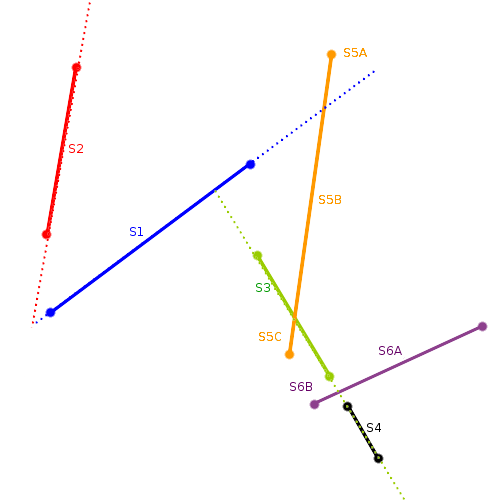
\includegraphics[scale=0.6]{bsp_ex_5.png}
\caption{Application de l'heuristique sur le nœud dont la droite est construite via $S3$}
\label{bsp_ex_5}
\end{figure}

La construction se poursuit récursivement pour donner l'arbre à la figure \ref{bsp_tree}.

\begin{figure}[H]
\centering
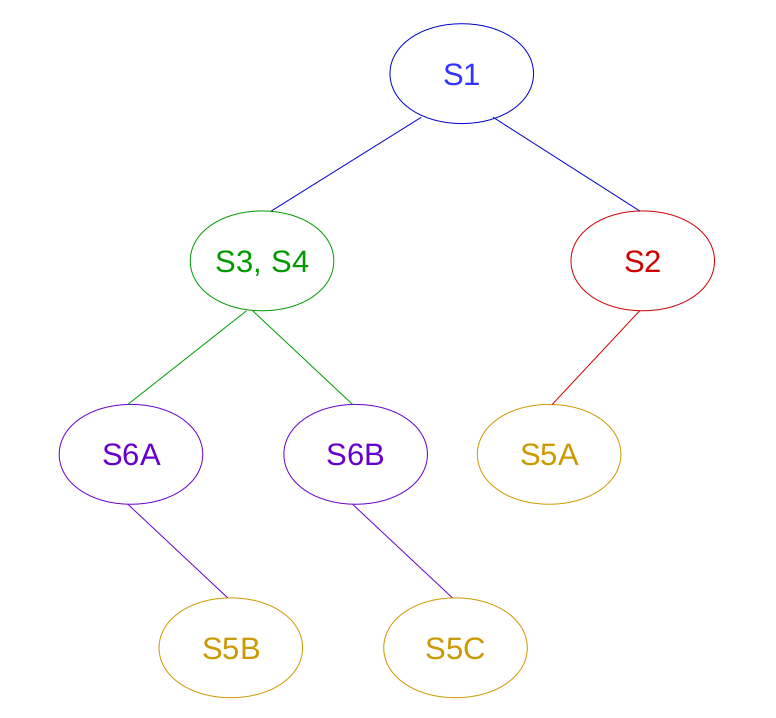
\includegraphics[scale=0.35]{bsp_ex_3.png}
\caption{Arbre BSP}
\label{bsp_tree}
\end{figure}

\paragraph{Pseudo-code}

Afin d'implémenter cette heuristique, nous utilisons principalement les deux algorithmes suivants :\\

\begin{itemize}
\item createTree : permet de lancer la création de l'arbre en initialisant la racine;
\item createRoot : assure la construction récursive de l'arbre à partir d'un nœud;
\end{itemize}\\
\bigskip

Notons que nous utilisons les conventions suivantes :\\

\begin{itemize}
\item La création d'un nœud nécessite 4 paramètres : fils droit, fils gauche, la liste de segments à traiter et la droite effectuant la séparation du plan (appelée \emph{splitting line}).
\item Rappelons qu'un nœud possède cinq attributs :
\begin{itemize}
	\item rightSon
	\item leftSon
	\item segmentsInHyperplane : liste des segments dans l'hyperplan défini par le droite de séparation du père.
	\item segmentsInLine : segments dans la ligne de séparation.
	\item line : tableau de trois doubles étant les coefficients a, b et c de l'équation de sa droite de séparation.
\end{itemize}
\item Un nœud possède entre autres les deux méthodes setLeftSon et setRightSon permettant d'ajouter respectivement un fils gauche et/ou un fils droit au nœud. 
\end{itemize}

\newpage

\begin{alltt}
\textbf{createTree}
Entrée : segList, liste de segments d'origine pour la création 
de l'arbre BSP (issue du fichier).
Sortie : racine de l'arbre BSP généré

1: \(line \leftarrow segList[0]\)
2: enlever \(segList[0]\) de \(segList\)
3: \(racine\) \(\leftarrow\) nouveau noeud (\(vide\), \(vide\), \(segList\), \(line\))
4: createRoot(\(racine\))
5: retourner \(racine\)
\end{alltt}

\begin{alltt}
\textbf{createRoot}
Entrée : noeud, étant un noeud incomplet de l'arbre BSP ne
disposant que de sa ligne de séparation et sa liste de
segments à traiter.
Sortie : /
Effet : ajoute les segments contenus dans la 
droite de séparation dans la liste adéquate.
Ajoute les fils au nœud s'il en a et dans ce cas 
appelle l'algorithme récursivement sur ces derniers en 
choisissant une nouvelle droite de séparation et en 
donnant les nouvelles listes de segments adaptées.

 1: si \(noeud\) non vide alors
 2:   pour chaque segment \(s\) dans \(noeud.segmentsInHyperplane\) faire
 3:     si \(s \in noeud.line\) alors
 4:       ajouter \(s\) à \(segmentsInLine\)
 5:       enlever \(s\) de \(segmentsInHyperplane\)
 6:       
 7:   créer les listes \(leftNodeSegments\) et \(rightNodeSegments\)
 8:   
 9:   pour chaque segment \(s\) dans \(noeud.segmentsInHyperplane\) faire
10:     si \(s\) est à droite de \(noeud.line\) alors
11:       ajouter \(s\) à \(rightNodeSegments\)
12:
13:     sinon si \(s\) est à gauche de \(noeud.line\) alors
14:       ajouter \(s\) à \(leftNodeSegments\)
15:
16:     sinon on est dans le cas où \(s\) intersecte \(noeud.line\) alors
17:       créer deux nouveaux segments \(s1\) et \(s2\)
18:       si \(s1\) est à droite de \(noeud.line\) alors
19:         ajouter \(s1\) à \(rightNodeSegments\)
20:         ajouter \(s2\) à \(leftNodeSegments\)
21:
22:       sinon
23:         ajouter \(s1\) à \(leftNodeSegments\)
24:         ajouter \(s2\) à \(rightNodeSegments\)
25:         
26:   si \(leftNodeSegments\) et \(rightNodeSegments\) sont non-vides alors
27:     \(line \leftarrow rightNodeSegments[0]\)
28:     enlever \(rightNodeSegments[0]\) de \(rightNodeSegments\)
29:     \(rightNode \leftarrow\) nouveau noeud (\(vide\), \(vide\), \(rightNodeSegments\), \(line\))
30:     setRightSon(\(rightNode\))
31:     \(line \leftarrow leftNodeSegments[0]\)
32:     enlever \(leftNodeSegments[0]\) de \(leftNodeSegments\)
33:     \(leftNode \leftarrow\) nouveau noeud (\(vide\), \(vide\), \(leftNodeSegments\), \(line\))
34:     setLeftSon(\(leftNode\));
35:     
36:   sinon si \(leftNodeSegments\) vide et \(rightNodeSegments\) non-vide alors
37:     \(line \leftarrow rightNodeSegments[0]\)
38:     enlever \(rightNodeSegments[0]\) de \(rightNodeSegments\)
39:     \(rightNode \leftarrow \) nouveau noeud (\(vide\), \(vide\), \(rightNodeSegments\), \(line\))
40:     setRightSon(\(rightNode\))
41:    
42:   sinon si \(leftNodeSegments\) non-vide et \(rightNodeSegments\) vide alors
43:     \(line \leftarrow leftNodeSegments[0]\)
44:     enlever \(leftNodeSegments[0]\) de \(leftNodeSegments\)
45:     \(leftNode \leftarrow \) nouveau noeud (\(vide\), \(vide\), \(leftNodeSegments\), \(line\))
46:     setLeftSon(\(leftNode\))
47:     
48:   createRoot(\(leftNode)\))
49:   createRoot(\(rightNode\))
\end{alltt}

Pour effectuer la création d'un arbre BSP avec l'heuristique "in-order" nous appelons simplement createTree avec la liste des segments devant former l'arbre. Cet algorithme va alors se charger d'initialiser le premier nœud en utilisant le premier segment de la liste comme droite de séparation. Ensuite l'algorithme createRoot est appelé avec ce premier nœud, c'est cet algorithme qui se charge ensuite de la construction récursive de l'arbre. \\

Tout d'abord, l'instruction 1 permet de ne faire fonctionner l'algorithme que s'il a du sens, c'est à dire que le nœud sur lequel il est appelé est non nul. Nous pouvons ensuite effectuer une analyse en deux parties : 

La première partie, constituée des instructions 2 à 25, consiste en la création de deux nouveaux hyperplans $s^+$ et $s^-$ en fonction de la "splitting line", ou droite de division de l'espace $s$ du nœud. On regarde d'abord si des segments de l'hyperplan du nœud sont contenus dans cette droite et, s'ils existent, on les ajoute à la liste des segments contenus dans la droite. Ensuite, avec les segments restants, on va regarder s'ils se situent à gauche ou à droite de la "splitting line", donc $s^+$ ou $s^-$ pour ensuite pouvoir les répartir correctement (dans le cas où il y a intersection, on crée deux nouveaux segments et on les ajoute au bon nouvel hyperplan en fonction de leur position). 

La seconde partie permet la création de la structure d'arbre en tant que telle, constituée des instructions 26 à 49. Elle va simplement attribuer au nœud un fils gauche et un fils droit si de tels fils existent. En effet, on peut se trouver dans le cas d'une feuille, ou on a juste un ou plusieurs segments dans $segmentsInLine$ qui définissent une "splitting line" mais aucuns segments dans "segmentsInHyperPlane". Nous pouvons aussi nous trouver dans le cas ou il n'y a aucun segment compris dans $s^+$ ou $s^-$, ce qui revient à ne pas avoir de fils droit ou gauche. La liste de segments correspondant au nœud, calculé dans la première partie, leur est attribué et une nouvelle droite de séparation (générée à partir du premier segment de cette liste) leur est donnée. Ensuite l'algorithme est appelé récursivement sur ces deux fils (pouvant résulter sur un appel récursif sur un fils Null qui sera écartée par l'instruction 1). 

\subsubsection{Heuristique "random"}

\paragraph{Méthode}

Cette heuristique utilise la même méthode que l'heuristique "in-order" pour la création de l'arbre BSP, à la seule différence près que la liste des segments est mélangée avant de commencer la construction. Ceci va donc changer l'ordre de création des lignes de séparation et donc la structure de l'arbre. Cette utilisation aléatoire du mélange de la liste a pour conséquence que l'algorithme n'est plus déterministe. La différence d'un point de vue algorithmique avec l'heuristique précédente étant nulle, nous ne attardons donc pas sur ce point. 

\paragraph{Pseudo-code}

L'implémentation de cette heuristique est identique à la précédente à l'exception d'une ligne effectuant le mélange de la liste des segments avant utilisation. On va donc ici mélanger la liste des segments, puis appeler l'algorithme précédent :

\begin{alltt}
\textbf{createTree}
Entrée : segList, liste de segments d'origine pour la création 
de l'arbre BSP
Sortie : racine de l'arbre BSP généré

1: \(inorder \leftarrow\) nouveau InOrderHeuristic()
2: mélanger \(segList\)
3: retourner inorder.createTree(\(segList\))
\end{alltt}

\subsubsection{Heuristique "free-splits"}

\paragraph{Méthode}

Afin d'expliquer au mieux cette heuristique, nous utiliserons également un exemple, représenté à la Figure \ref{scene_splits}. \\

Cette heuristique se veut plus réfléchie que la simple utilisation, dans un ordre aléatoire ou non, des segments pour la définition de nouveaux plans. Nous allons donc étudier ici le cas particulier des "free-splits", ce dernier n'apparaissant que dans des circonstances bien précises, recréées ici dans l'exemple. Notons que cette heuristique se base sur une liste de segments ordonnés de manière aléatoire, néanmoins, pour les besoins de l'exemple nous supposerons que l'algorithme traite les segments dans l'ordre où ceux-ci ont été définis. En effet, si nous traitons les segments dans un ordre aléatoire, il se pourrait que nous soyons en présence d'une situation ne disposant pas de "free-split".

\begin{figure}[!h]
\centering
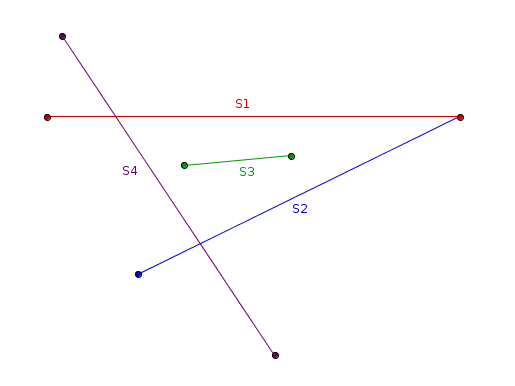
\includegraphics[scale=0.5]{free_splits_2.png}
\caption{Scène 2D}
\label{scene_splits}
\end{figure}

Exécutons pas à pas l'algorithme et définissons à l'aide de l'exemple la notion de "free-split". \\

Nous pouvons observer que cette scène est composée de 4 segments. Imaginons que nous avons déjà construit une partie de l'arbre BSP avec S1 et S2, nous remarquons alors que ces deux segments coupent S4, ce qui divise S4 en trois nouveaux segments (nommés S4A, S4B et S4C dans la Figure \ref{heuristic_splits}). A cette étape nous avons déjà la partie gauche de l'arbre construite avec S4A en tant que feuille (voir Figure \ref{split_bsp}). Il reste alors à construire le côté droit à partir de S2. S4C étant tout seul de son côté, le choix se porte alors entre S3 et S4B comme base pour une nouvelle droite. Or étant donné que S4B est déjà intersecté par deux droites, l'utiliser comme nouvelle droite ne causera pas de nouvelle fragmentation lors de la création du noeud ! C'est ce que l'on appelle la notion de "free-splits", c'est à dire utiliser des segments déjà intersectés par deux droites existantes pour définir de nouveaux plans, car ceux-ci, par conséquent ne fragmenteront plus aucun segment. Ce qui donc est avantageux au niveau de la quantité de segments qui est alors censée être réduite.\\

Notons que lorsqu'aucun "free-split" n'est présent, c'est l'algorithme classique "random" de création d'arbre BSP qui est d'application. 

\begin{figure}[!h]
\centering
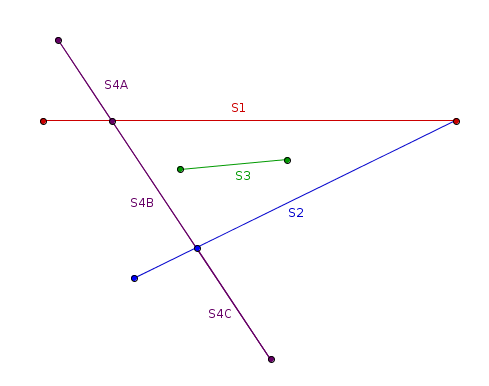
\includegraphics[scale=0.5]{free_splits_1.png}
\caption{Application de l'heuristique}
\label{heuristic_splits}
\end{figure}


\begin{figure}[!h]
\centering
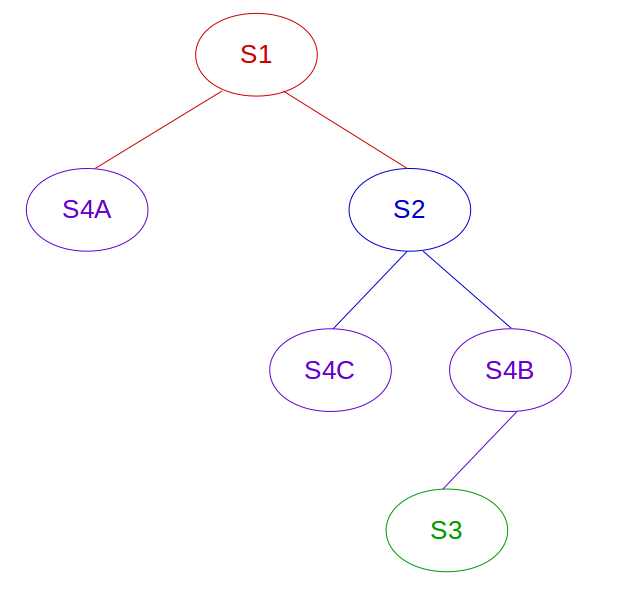
\includegraphics[scale=0.4]{free_splits_3.png}
\caption{Arbre BSP}
\label{split_bsp}
\end{figure}

\paragraph{Implémentation}

L'implémentation de l'heuristique des "free-splits" paraît à première vue fort semblable par rapport à celle "inorder", ce qui est normal étant donné qu'elles possèdent la même structure, "free-splits" n'apportant que quelques améliorations se basant sur des conditions supplémentaires. Nous allons donc ici présenter un pseudo-code très semblable au précédent, c'est pourquoi les numéros de lignes présentant un changement seront mises en gras.\\

Pour les besoins de l'heuristique nous introduisons les attributs suivants aux objets de type segment : un booléen isIntersected indiquand si le segment a déjà été intersecté ou non, un tableau de deux nombres nommé intersection contenant cette intersection si elle existe et un booléen isFreeSplit indiquant si le segment est un "free-split". Notons également les deux abréviations suivantes : a et b pour désigner les deux extrémités du segment.\\

Notons bien qu'afin de comprendre sans ambiguïté les lignes 20,25,27 et 30, nous admettons que lorsque nous réalisons une coupure au niveau d'un segment par une droite, celle-ci se fait au niveau de l'extrémité b pour les nouveaux segments. 

\begin{alltt}
\textbf{createTree}
Entrée : segList, liste de segments d'origine pour la création 
de l'arbre BSP
Sortie : racine de l'arbre BSP généré

\textbf{1:} mélanger \(segList\)
2: \(line \leftarrow segList[0]\)
3: enlever \(segList[0]\) de \(segList\)
4: \(racine\) \(\leftarrow\) nouveau noeud (\(vide\), \(vide\), \(segList\), \(line\))
5: createRoot(\(racine\))
6: retourner \(racine\)
\end{alltt} 

\begin{alltt}
\textbf{createRoot}
Entrée : noeud, étant un noeud incomplet de l'arbre BSP ne
disposant que de sa ligne de séparation et sa liste de
segments contenus dans son hyperplan.
Sortie : /
Effet : ajoute les fils au noeud s'il en a et dans ce cas 
appelle l'algorithme récursivement sur ces derniers en 
choisissant une nouvelle droite de séparation et en 
donnant les nouvelles listes de segments adaptées.

 1: si \(noeud\) non vide alors
 2:   pour chaque segment \(s\) dans \(noeud.segmentsInHyperplane\) faire
 3:     si \(s \in noeud.line\) alors
 4:       ajouter \(s\) à \(segmentsInLine\)
 5:       enlever \(s\) de \(segmentsInHyperplane\)
 6:       
 7:   créer les listes \(leftNodeSegments\) et \(rightNodeSegments\)
 8:   
 9:   pour chaque segment \(s\) dans \(noeud.segmentsInHyperplane\) faire
10:     si \(s\) est à droite de \(noeud.line\) alors
11:       ajouter \(s\) à \(rightNodeSegments\)
12:
13:     sinon si \(s\) est à gauche de \(noeud.line\) alors
14:       ajouter \(s\) à \(leftNodeSegments\)
15:
16:     sinon on est dans le cas où \(s\) intersecte \(noeud.line\) alors
17:       créer deux nouveaux segments \(s1\) et \(s2\)
18:
\textbf{20:}		      si \(s\) est intersecté et intersection \(=s1.a\) alors
\textbf{21:}		        \(s1\) devient un free-split
\textbf{22:}		    
\textbf{23:}		      sinon
\textbf{24:}		        \(s1\) devient intersecté
\textbf{25:}		        \(s1.intersection\) = \(s1.b\)
\textbf{26:}		    
\textbf{27:}		      si \(s\) est intersecté et intersection \(=s2.a\) alors
\textbf{28:}		        \(s2\) devient un free-split
\textbf{29:}		    
\textbf{30:}		      sinon
\textbf{31:}		        \(s2\) devient intersecté
\textbf{32:}		        \(s2.intersection\) = \(s2.b\)
33:		
34:       si \(s1\) est à droite de \(noeud.line\) alors
35:         ajouter \(s1\) à \(rightNodeSegments\)
36:         ajouter \(s2\) à \(leftNodeSegments\)
37:
38:       sinon
39:         ajouter \(s1\) à \(leftNodeSegments\)
40:         ajouter \(s2\) à \(rightNodeSegments\)
41:   
\textbf{42:}	  \(fsLeft = faux\)
\textbf{43:}	  \(fsRight = faux\)
\textbf{44:}      
\textbf{45:}   si taille de \(leftNodeSegments < 1\)
\textbf{46:}     pour chaque segment \(s\) dans \(leftNodeSegments\) faire
\textbf{47:}       si \(s\) est free-split
\textbf{48:}         \(fsLeft = true\)
\textbf{49:}         enlever \(s\) de \(leftNodeSegments\)
\textbf{50:}         \(leftNode \leftarrow \) nouveau noeud (\(vide\), \(vide\), \(leftNodeSegments\), \(s\))
\textbf{51:}         setLeftSon(\(leftNode\))
\textbf{52:}            
\textbf{53:}    si taille de \(rightNodeSegments < 1\)
\textbf{54:}      pour chaque segment \(s\) dans \(rightNodeSegments\) faire
\textbf{55:}        si \(s\) est free-split
\textbf{56:}          \(right = true\)
\textbf{57:}          enlever \(s\) de \(rightNodeSegments\)
\textbf{58:}          \(rightNode \leftarrow \) nouveau noeud (\(vide\), \(vide\), \(rightNodeSegments\), \(s\))
\textbf{59:}          setrightSon(\(rightNode\))
60:
61:   si \(leftNodeSegments\) et \(rightNodeSegments\) sont non-vides alors
\textbf{62:}	    si \(fsRight\) est faux
63:       \(line \leftarrow rightNodeSegments[0]\)
64:       enlever \(rightNodeSegments[0]\) de \(rightNodeSegments\)
65:       \(rightNode \leftarrow\) nouveau noeud (\(vide\), \(vide\), \(rightNodeSegments\), \(line\))
66:       setRightSon(\(rightNode\))
67
\textbf{68:}	    si \(fsLeft\) est faux
69:       \(line \leftarrow leftNodeSegments[0]\)
70:       enlever \(leftNodeSegments[0]\) de \(leftNodeSegments\)
71:       \(leftNode \leftarrow\) nouveau noeud (\(vide\), \(vide\), \(leftNodeSegments\), \(line\))
72:       setLeftSon(\(leftNode\));
73:     
\textbf{74:}   sinon si \(leftNodeSegments\) vide et \(rightNodeSegments\) non-vide et
\textbf{75:}   \(fsLeft\) est faux alors
76:     \(line \leftarrow rightNodeSegments[0]\)
77:     enlever \(rightNodeSegments[0]\) de \(rightNodeSegments\)
78:     \(rightNode \leftarrow \) nouveau noeud (\(vide\), \(vide\), \(rightNodeSegments\), \(line\))
79:     setRightSon(\(rightNode\))
80:    
\textbf{81:}   sinon si \(leftNodeSegments\) non-vide et \(rightNodeSegments\) vide 
\textbf{82:}   et \(fsRight\) est faux alors
83:     \(line \leftarrow leftNodeSegments[0]\)
84:     enlever \(leftNodeSegments[0]\) de \(leftNodeSegments\)
85:     \(leftNode \leftarrow \) nouveau noeud (\(vide\), \(vide\), \(leftNodeSegments\), \(line\))
86:     setLeftSon(\(leftNode\))
87:     
88:   createRoot(\(leftNode)\))
89:   createRoot(\(rightNode\))
\end{alltt}

Au niveau du code présent aux lignes 20-32, il s'agit de la recherche de free-splits. En effet ceux-ci peuvent se créer lorsqu'il y a une coupure d'un segment par une droite. Ce dernier, si déjà intersecté précédemment, présente alors un free-split sur un de ses sous-segments récemment créés. C'est ce que nous réalisons aux lignes 20-21 et 27-28, en vérifiant bien si nous nous trouvons sur le bon sous-segment. Par contre si le segment original n'a pas encore été intersecté, nous marquons les deux sous-segments comme intersectés et conservons dans une variable le point d'intersection. \\

Pour les instructions 42-59, il s'agit simplement d'une vérification permettant de savoir si des free-splits sont présent dans la liste des segments pour le fils gauche et le fils droit. Si c'est le cas, le noeud est créé avec le segment résultant du free-split comme base pour une nouvelle droite de séparation, un booléen est mis à vrai et il n'y aura donc pas de choix aléatoire comme dans l'heuristique précédente. Et cela grâce aux conditions ajoutée en 62,68,74-75 et 81-82. Si aucun free-split n'est trouvé, le premier segment de l'hyperplan en question est choisi comme nouvelle "splitting-line", comme dans l'heuristique précédente. 

\newpage

\section{Algorithme du peintre}

Notre implémentation de l'algorithme du peintre est similaire à celle présentée dans le livre de référence. Son principe est le suivant : chaque nœud de l'arbre BSP est parcouru dans un certain ordre et les segments qu'il contient sont alors affichés si ils sont visibles par le point de vue.

\subsection{Structures de données}
Les algorithmes présentés dans cette section utilisent les structures de données Segment pour représenter les segments, BSPNode pour représenter les arbres et listes chaînées pour stocker les segments comme elles ont été présentées dans la section \textit{1.2}

\subsubsection{Point de vue}
La structure de données Pov (\emph{Point Of View}) permet de représenter un point de vue. Celui-ci contient plusieurs attributs utiles pour l'algorithme du peintre :\\

\begin{itemize}
	\item \emph{position} le point de départ du point de vue, stocké sous forme d'un tableau de doubles à deux dimensions.
	\item \emph{line1} le premier vecteur qui définit le point de vue, stocké sous forme d'un objet qui comprend les deux points composant ce segment.
	\item \emph{line2} le deuxième vecteur qui définit le point de vue, stocké sous forme d'un objet qui comprend les deux points composant ce segment.
	\item \emph{directorVector} le vecteur directeur du point de vue, reliant le point stocké dans \emph{position} et le point entre les extrémités des deux segments qui définissent le point de vue. Ce vecteur directeur est essentiellement la bissectrice du point de vue et est stocké de la même façon que précédemment.
	\item \emph{projectionLine} la ligne sur laquelle seront projetés les segments vu par le point de vue, stockée de la même façon que précédemment.
\end{itemize}

\subsection{Algorithme principal}
\subsubsection{Pseudo-code}
Le pseudo code suivant part du principe que les segments sont directement affichés par l'algorithme du peintre. En réalité, l'algorithme du peintre ajoute les segments à dessiner dans le bon ordre dans une liste chaînée qui sera ensuite utilisée par l'interface graphique. Ce détail d'implémentation ne changeant rien à la complexité et gênant la bonne compréhension de l'algorithme, nous l'ignorons ici.\\

\newpage

\begin{lstlisting}
paintersAlgorithm
Entrées : N la racine d'un arbre BSP, P un point de vue
Sortie : / (les segments sont dessinés dans le bon ordre)

 1: si !vide(N) alors
 2
 3:    si feuille(N) alors
 4:       drawSegments($N_{liste}$)
 5:
 6:    si $P \in N_{s^+}$ alors
 7:       paintersAlgorithm($N_{filsGauche}$,$P$)
 8:       scanConvert($N_{liste}$)
 9:       paintersAlgorithm($N_{filsDroit}$,$P$)
10:
11:    si $P \in N_{s^-}$ alors
12:       paintersAlgorithm($N_{filsDroit}$,$P$)
13:       scanConvert($N_{liste}$)
14:       paintersAlgorithm($N_{filsGauche}$,$P$)
15:
16:    sinon
16:       paintersAlgorithm($N_{filsDroit}$,$P$)
17:       paintersAlgorithm($N_{filsGauche}$,$P$)
\end{lstlisting}

\subsubsection{Méthode}
Cet algorithme permet de parcourir l'arbre BSP pour afficher les segments par ordre de distance avec le point de vue (les segments les plus éloignés étant dessinés en premier).\\

Nous vérifions tout d'abord si la racine $N$ de l'arbre n'est pas vide Ce cas peut résulter d'un appel récursif sur l'algorithme avec un nœud $N$ qui n'a pas de fils gauche et/ou de fils droit. L'appel se fera donc avec un nœud null et ne résultera en aucun calcul.\\

Ensuite, il est évident que si le nœud $N^$ est une feuille, nous ne pouvons plus parcourir récursivement l'arbre et nous appelons donc la méthode \textbf{scanConvert} qui permet d'afficher les segments contenus dans le nœud $N$ si ceux-ci sont visibles par le point de vue $P$. Il est utile de rappeler que les segments potentiellement affichés sont ceux contenus dans la droite de séparation du nœud $N$, stockés dans $N_{liste}$.\\

Si le point de vue $P$ appartient à $N_{s^+}$, nous voulons d'abord afficher les segments plus distants que ceux de $N_{liste}$, 
ceux si seront ceux du fils gauche qui appartient à $N_{s^-}$ et possède donc des segments plus distants du point de vue comme détaillé sur la figure \ref{ordre_1}. Le même principe s'applique pour le cas ou $P$ appartient à $N_{s^-}$.

\begin{figure}[!h]
\centering
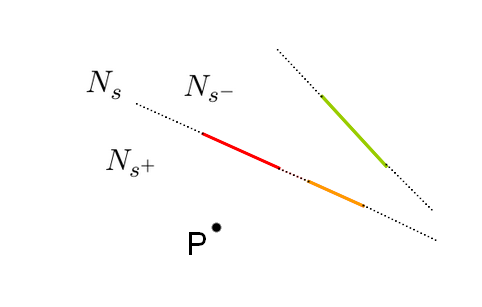
\includegraphics[scale=0.5]{painter_ordre_1.png}
\caption{Ordre de parcours si $P \in N_{s^+}$ }
\label{ordre_1}
\end{figure}

Si $P$ n'appartient pas à $N_{s^+}$ ni à $N_{s^-}$ alors $P \in N_s$ et les segments de $N_{liste}$ ne doivent pas être affichés car ils ne sont forcément pas visible par le point de vue et le parcours est continué.

\subsubsection{Complexité}
La complexité dans le pire des cas d'un algorithme sur un arbre se fait de la manière suivante :
\begin{center}
(nombre de nœuds visités $\times$ complexité pour un nœud) \\
$+$ \\
(nombre de références vides $\times$ complexité pour une référence vide)
\end{center}
Il est utile de rappeler qu'un arbre binaire possédant $n$ nœuds a $n+1$ références vides.\\

Nous remarquons d'abord que l'algorithme du peintre est un parcours d'un arbre BSP dans un certain ordre. Tous les nœuds de l'arbre sont donc parcourus. Pour chaque nœud, la méthode \textbf{scanConvert} est appelée sauf si le point de vue est sur la droite de séparation de ce nœud. Dans le pire des cas, nous aurons toujours un appel à \textbf{scanConvert} pour chaque nœud.\\

Comme indiqué dans la section $2.3.3$, la complexité de \textbf{scanConvert} pour un nœud dépend de la taille de la liste de segments de ce nœud. Un appel à cette méthode pour une liste entrée de taille $m$ sera en $O(m)$. \\

Tout ceci nous permet de déduire que la complexité de l'algorithme du peintre dépend du nombre total de segments contenu dans l'arbre. En effet, chaque nœud de l'arbre sera visité et tous les segments contenus dans sa droite de séparation seront parcourus. Pour un arbre contenant $n$ nœuds et de taille $m$ (donc contenant $m$ segments), nous obtenons la complexité suivante :\\

Complexité pour chaque nœud :\\
Chaque nœud sera noté $k_1, k_2, ... , k_n$;\\
Pour chaque nœud, la taille de sa liste de segments sera notée $t_1, t_2, ... , t_n$ et nous savons que $t_1 + t_2 + ... + t_n = \text{taille de l'arbre}$\\
Chaque appel sur un nœud $k_i$ aura une complexité en $O(t_i)$. En effet chacun des segments contenus dans ce nœud seront parcourus.

L'algorithme est appelé sur les $n$ nœuds de l'arbre, donc sur $k_1, k_2, ... , k_n$ et chacun de ces appels aura une complexité en $O( t_1), O(t_2), ... , O(t_n)$.\\
La complexité totale pour l'arbre sera alors de $O(t_1 + t_2 + ... + t_n) = O(m)$. La complexité de l'algorithme du peintre dépend donc de la taille de l'arbre BSP.

\subsection{Algorithme de projection}

\subsubsection{Pseudo-code}

Les figures \ref{painter_notations} et \ref{painter_notations_2} rendent compte des notations utilisées dans l'algorithme.
\\
\begin{figure}[!htbp]
  \centering
  \begin{minipage}[b]{0.4\textwidth}
    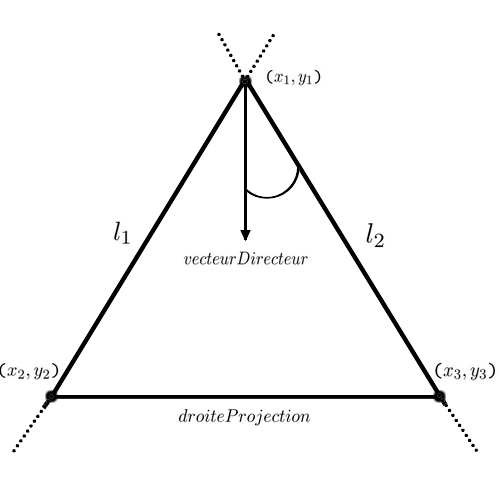
\includegraphics[width=\textwidth]{painter_notations.png}
    \caption{Notations du point de vue}
		\label{painter_notations}
  \end{minipage}
  \hfill
  \begin{minipage}[b]{0.4\textwidth}
    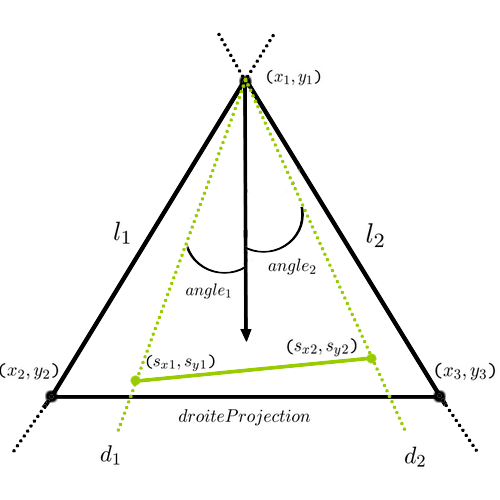
\includegraphics[width=\textwidth]{painter_notations_2.png}
    \caption{Notations avec segment $s$}
		\label{painter_notations_2}
  \end{minipage}
\end{figure}
\\

\begin{lstlisting}
scanConvert
Entrées : L une liste d'objets segments
Sortie : / (les segments sont dessinés)
\end{lstlisting}

\newgeometry{margin=0.4in}

\begin{lstlisting}
 1: $l_1$ $\leftarrow$ calcDroite($x_1,y_1,x_2,y_2$)
 2: $l_2$ $\leftarrow$ calcDroite($x_1,y_1,x_3,y_3$)
 3: $limite_1$ $\leftarrow$ ($x_2,y_2$)
 4: $limite_2$ $\leftarrow$ ($x_3,y_3$)
 5: $position$ $\leftarrow$ ($x_1,y_1$)
 6: $vecteurDirecteur$ $\leftarrow$ pointDeVue.vecteurDirecteur
 7: $demisAngle$ $\leftarrow$ calcAngle($l_1$, $vecteurDirecteur$)
 8: $droiteProjection$ $\leftarrow$ calcDroite($x_2,y_2,x_3,y_3$)
 9: 
10: pour chaque segment $s$ dans $L$ faire
11:   $d_1$ $\leftarrow$ calcDroite($x_1,y_1,s_x_1,s_y_1$)
12:   $d_2$ $\leftarrow$ calcDroite($x_1,y_1,s_x_2,s_y_2$)
13:   $angle_1$ $\leftarrow$ calcAngle($vecteurDirecteur$, $d_1$)
14:   $angle_2$ $\leftarrow$ calcAngle($vecteurDirecteur$, $d_2$)
15:
16:   si $|angle_1| \leq |demisAngle|$ et $|angle_2| \leq |demisAngle|$ alors
17:      $i_1$ $\leftarrow$ calcInter($d_1$,$droiteProjection$)
17:      $i_2$ $\leftarrow$ calcInter($d_2$,$droiteProjection$)
18:      dessiner($i_1,i_2$,$s_{couleur}$)
19:
20:   sinon si $|angle_1| \leq |demisAngle|$ et $|angle_2| > |demisAngle|$ alors
21:   |   $i_1$ $\leftarrow$ $s$.calcPosition($l_1$)
22:   |   $i_2$ $\leftarrow$ $s$.calcPosition($l_2$)
23:   |
24:   |   si !$i_1$=gauche et !$i_1$=droite et !$i_2$=gauche et !$i_2$=droite alors
25:   |   |   $norme_1$ $\leftarrow$ calcNorme($s_x_1,s_y_1,i_1_x,i_1_y$)
26:   |   |   $norme_2$ $\leftarrow$ calcNorme($s_x_1,s_y_1,i_2_x,i_2_y$)
27:   |   |   
28:   |   |   si $min(norme_1,norme_2)=norme_1$ alors
29:   |   |   |   $j_1$ $\leftarrow$ calcInter($d_1$,$droiteProjection$)
30:   |   |   |   dessiner($j_1,limite_1$,$s_{couleur}$)
31:   |   |   |
32:   |   |   sinon
33:   |   |   |   $j_1$ $\leftarrow$ calcInter($d_1$,$droiteProjection$)
34:   |   |   |   dessiner($j_1,limite_2$,$s_{couleur}$)
35    |   |   |
36:   |   sinon si !$i_1$=gauche et !$i_1$=droite alors
37:   |   |   $j_1$ $\leftarrow$ calcInter($d_1$,$droiteProjection$)
38:   |   |   dessiner($j_1,limite_1$,$s_{couleur}$)
39    |   |
40:   |   sinon si !$i_2$=gauche et !$i_2$=droite alors
41:   |   |   $j_1$ $\leftarrow$ calcInter($d_1$,$droiteProjection$)
41:   |   |   dessiner($j_1,limite_2$,$s_{couleur}$)
42:   |   |
43:   sinon si $|angle_1| > |demisAngle|$ et $|angle_2|\leq |demisAngle|$ alors
44:      Cas semblable au cas précédent
45:
46:   sinon si $|angle_1|>|demisAngle|$ et $|angle_2|>|demisAngle|$ et ( ($angle_1\geq 0$ et $angle_2<0$)
47:   |         ou ($angle_1 <0$ et $angle_2\geq 0$) ) et ( ($angle_1<90$) ou ($angle_2<90$) ) alors
48:   |
49:   |   $i_1$ $\leftarrow$ $s$.calcPosition($l_1$)
50:   |   $i_2$ $\leftarrow$ $s$.calcPosition($l_2$)
51:   |
52:   |   si !$i_1$=gauche et !$i_1$=droite et !$i_2$=gauche et !$i_2$=droite alors
53:   |      $liste$ $\leftarrow$ nouvelleListe()
54:   |      $s'$ $\leftarrow$ Segment($i_1$,$i_2$,$s_{couleur}$)
54:   |      $L'$.ajouterSegment($s'$)
55:   |      scanConvert($L'$)
\end{lstlisting}
\restoregeometry

\subsubsection{Méthode}
Dans cette section, nous détaillerons le fonctionnement général de l'algorithme ainsi qu'un exemple.\\

Nous connaissons les valeurs de $(x_1,y_1)$, $(x_2,y_2)$, $(x_3,y_3)$ grâce au point de vue, ceci nous permet de calculer les droites $l_1$ et $l_2$, le vecteur directeur (qui joint $(x_1,y_1)$ au point situé entre $(x_2,y_2)$ et $(x_3,y_3)$), le segment sur lequel nous projetons la vue relie les deux points $(x_2,y_2)$, $(x_3,y_3)$ qui deviennent alors les $limites$ de ce segment (et aussi les projections de tout point sur $l_1$ et $l_2$). Nous calculons aussi le "demis angle" qui est l'angle entre le vecteur directeur et la droite $l_1$. Ceci nous donne le demis angle de vue (lignes 1 à 8). La situation de base est détaillée dans les figures \ref{exp_1} et \ref{exp_2}.

\begin{figure}[!h]
\centering
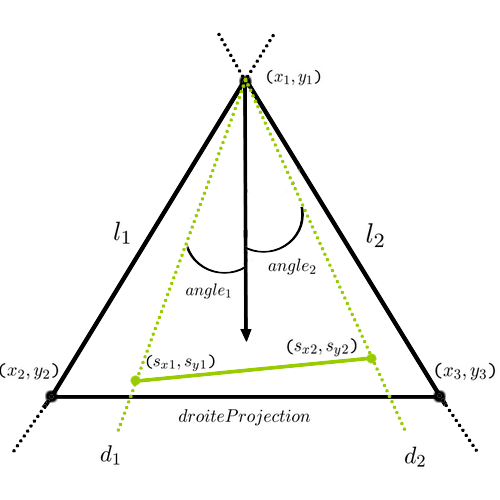
\includegraphics[scale=0.4]{painter_notations_2.png}
\caption{Notations avec segment $s$}
\label{exp_1}
\end{figure}
\newline
\begin{figure}[!h]
\centering
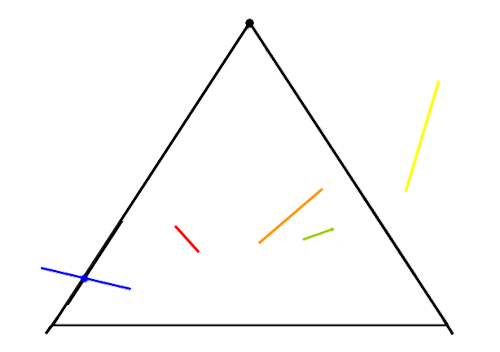
\includegraphics[scale=0.4]{base.png}
\caption{Scène de base}
\label{exp_2}
\end{figure}

\newpage

Pour chaque segment dans la liste, nous allons déterminer si celui-ci est visible par le point de vue (entièrement ou non) et l'afficher si c'est le cas.\\

Pour chaque segment, nous calculons les droites partant du point du vue et allant jusqu'aux deux extrémités de ce segment ainsi que les angles que ces droites forment avec le vecteur directeur (lignes 10 à 14). Ces angles nous permettent de déterminer si le segment est bien compris dans la vue ou non. Les droites en pointillé sur la figure \ref{exp_3} montrent cette situation (les angles ne sont pas représentés).

\begin{figure}[H]
\centering
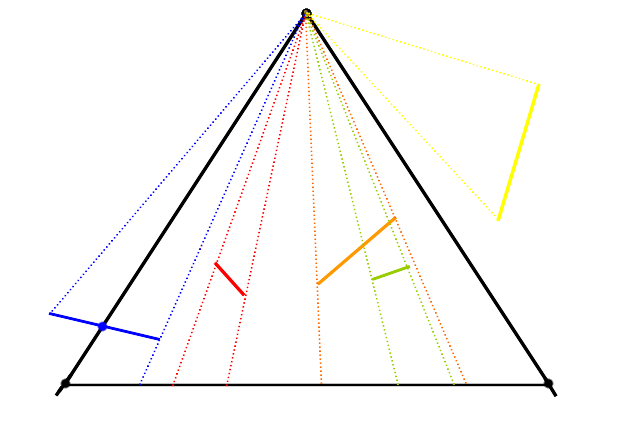
\includegraphics[scale=0.5]{inter.png}
\caption{Scène avec calcul des droites}
\label{exp_3}
\end{figure}

Si, pour un segment, ses deux angles calculés comme présenté ci-dessus sont plus petits que le demis angle, il est évident que le segment est complètement compris dans la vue. Nous l'affichons donc en entier. Pour ce faire nous projetons ses extrémités sur la droite de projection, ce qui revient à calculer l'intersection entre les droites qui relient le point de vue aux extrémités du segment et le segment sur lequel on veut projeter (lignes 16 à 18). Nous dessinons donc le segment reliant ces deux nouvelles intersections comme sur la figure \ref{cas1}.

\begin{figure}[H]
\centering
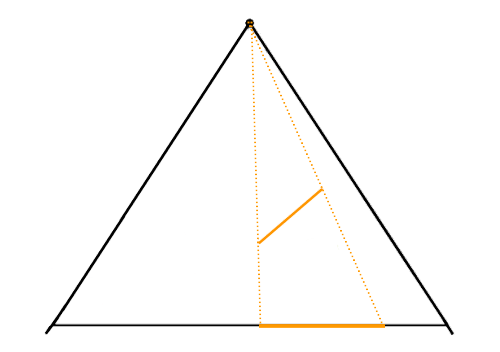
\includegraphics[scale=0.5]{cas1.png}
\caption{Cas du segment complètement dans la projection}
\label{cas1}
\end{figure}

Si un des deux angles est plus grand que le demis angle et l'autre plus petit, nous savons qu'une des deux extrémités du segment est dans la vue. Cette extrémité est celle qui forme la droite dont l'angle avec le vecteur directeur est plus petit que le demis angle. Nous devons dès lors déterminer l'autre extrémité du segment à projeter, qui se trouvera sur une des droites $l_1$ ou $l_2$ (le segment original étant coupé par une de ces droites). Pour déterminer cela, nous procédons comme suit :\\

Nous calculons la position du segment par rapport aux droites $l_1$ et $l_2$ (qui peut nous donner trois résultats : une intersection, à gauche de la droite ou à droite de la droite) et nous en déduirons la position de la deuxième extrémité du segment à projeter (lignes 21 et 22). \\

Si nous obtenons deux intersections, nous avons le cas particulier où le segment intersecte $l_1$ ou $l_2$ devant le point de vue et $l_2$ ou $l_1$ derrière le point de vue. Cette situation est représentée sur la figure \ref{exp_4}. Pour déterminer l'intersection $i_1$ ou $i_2$ qui nous intéresse (celle devant le point de vue), nous calculons la norme du vecteur reliant l'extrémité du segment qui est dans la vue et cette intersection $i_1$ ou $i_2$. Il est évident que la norme la plus petite est celle avec la bonne intersection (car si l'intersection est devant le point de vue, la norme sera moins grande car le point d'intersection sera plus proche de l'extrémité du segment). Nous savons ainsi si la ligne $l_1$ ou $l_2$ intersecte le segment. La deuxième extrémité du segment à projeter est donc sur cette ligne $l_1$ ou $l_2$. Dans le but de dessiner ce segment, nous en calculons les projections. Nous remarquons que la projection de l'extrémité qui est une intersection avec $l_1$ ou $l_2$ sera une des limites, car comme dit précédemment, la projection d'un point sur $l_1$ ou $l_2$ est respectivement $limite_1$ et $limite_2$ (lignes 24 à 34).\\

\begin{figure}[H]
\centering
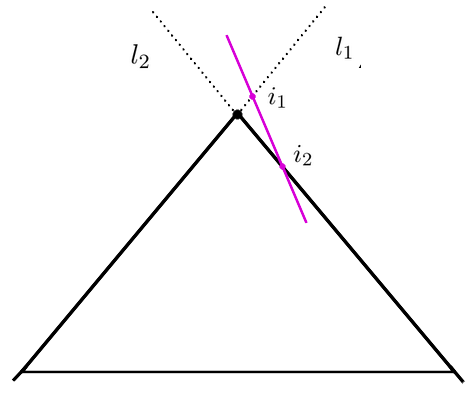
\includegraphics[scale=0.5]{casSpecial1.png}
\caption{Cas particulier où il y a deux intersections}
\label{exp_4}
\end{figure}

Si nous n'avons qu'une seule intersection avec $l_1$ ou $l_2$, la ligne $l_1$ ou $l_2$ qui intersecte le segment nous dit quel sera la deuxième extrémité du segment à projeter. En effet, si nous n'avons qu'une seule intersection avec $l_1$ ou $l_2$, nous savons que cette intersection sera la deuxième extrémité et sa projection sera donc $limite_1$ ou $limite_2$. Le segment bleu sur la figure \ref{cas2} montre cette situation ou $i_1$ nous donne un point d'intersection, ce qui nous permet de savoir que la ligne $l_1$ intersecte le segment. L'angle nous avait permis de savoir que le point ($s_{x_2},s_{y_2}$) du segment bleu $s$ était dans la vue. Le segment a dessiner ira donc de $limite_1$ à la projection de ($s_{x_2},s_{y_2}$) sur le segment de projection (lignes 36 à 41).\\

\begin{figure}[H]
\centering
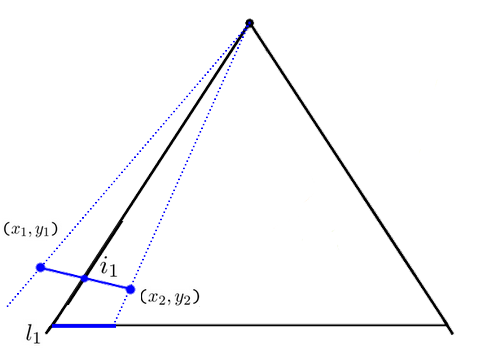
\includegraphics[scale=0.5]{cas2.png}
\caption{Cas ou le segment est coupé par $l_1$}
\label{cas2}
\end{figure}

Enfin, si nous avons deux angles plus grands que demis angle, qu'on a une droite qui relie le point de vue aux extrémités du segment de chaque coté du point de vue et qu'on moins une de ces droites est devant le point de vue (c'est à dire forme un angle inférieur à 90 degrés avec le vecteur directeur), il est possible que le segment coupe complètement le point de vue. Dès lors, nous calculons les intersections avec $l_1$ et $l_2$. Si nous obtenons deux intersections, le segment coupé reliera ces deux intersections et la méthode sera appelée récursivement sur ce segment coupé (lignes 46 à 55). Ceci débouche sur deux cas :\\

\begin{itemize}
	\item Le segment coupait bien le point de vue, le segment coupé sur lequel l'appel récursif est effectué est donc complètement compris dans le point de vue et sera affiché par le premier cas (figure \ref{exp_5}).
	\item Le segment coupait les deux droites derrière le point de vue, le segment coupé sur lequel l'appel récursif est effectué est n'est donc pas contenu dans le point de vue. Il ne passera dans aucuns cas et ne sera pas affiché (figure \ref{exp_6}).
\end{itemize}

\begin{figure}[H]
\centering
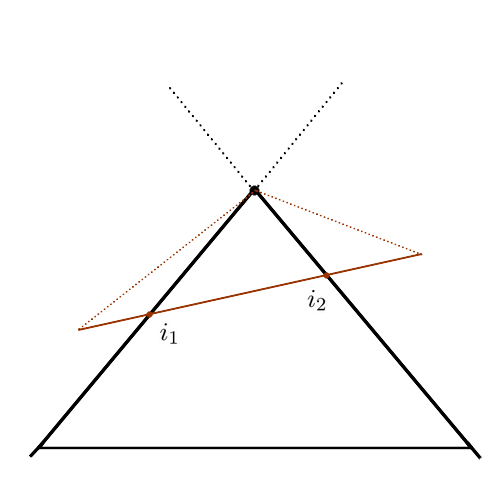
\includegraphics[scale=0.4]{casSpecial2.png}
\caption{Cas normal ou le segment coupe le point de vue et sera affiché}
\label{exp_5}
\end{figure}

\begin{figure}[H]
\centering
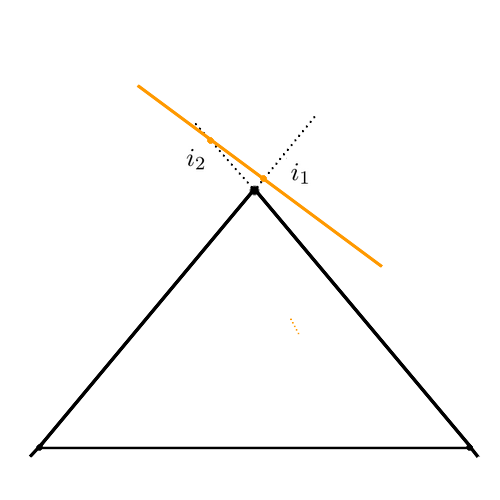
\includegraphics[scale=0.4]{casSpecial3.png}
\caption{Cas particulier ou le segment coupe les deux droites derrière le point de vue et ne sera pas affiché}
\label{exp_6}
\end{figure}

Grâce à l'ordre des appels sur cette méthode donné par l'algorithme du peintre, nous obtenus ce que voit le point de vue suite au traitement de tous les segments de l'arbre BSP comme montré sur la figure \ref{algofini}.

\begin{figure}[H]
\centering
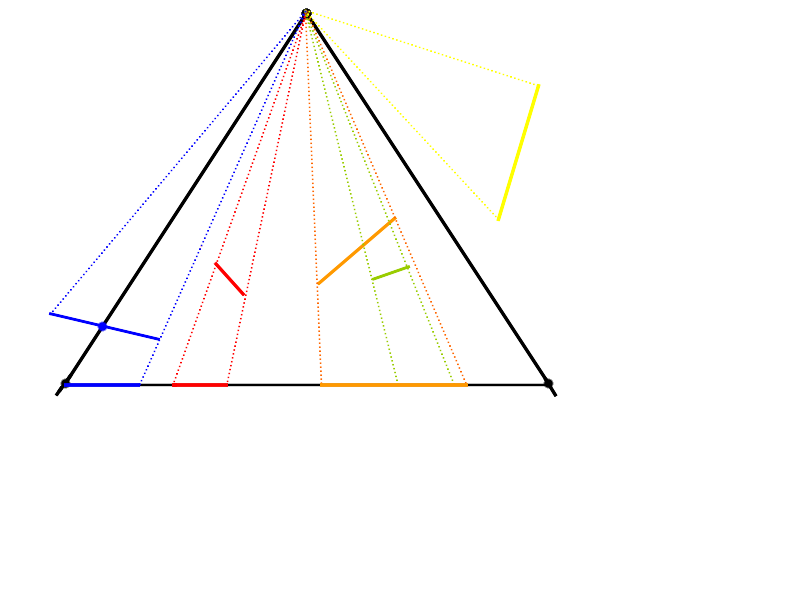
\includegraphics[scale=0.4]{fini.png}
\caption{Projection terminée telle qu'observée par le point de vue}
\label{algofini}
\end{figure}

\subsubsection{Complexité}
Les calculs effectués dans cette méthode sont en O($m$) avec $m$ le nombre de segments contenus dans la liste de segments pris en entrée. Dans le pire des cas, chaque segment traverse complètement le point de vue et nécessite un deuxième appel récursif sur la méthode \textbf{scanConvert}. Chaque segment de la liste résulte en deux appels de la méthode, donnant une complexité en O(2$m$) = O(m).

\section{Tests et Résultats}
L'algorithme du peintre parcourant tous les noeuds de l'arbre BSP ainsi que tous les segments contenus dans la ligne de séparation de l'espace de ce noeud, il est naturel que le temps d'exécution de l'algorithme dépendra du nombre de noeuds de l'arbre ainsi que du nombre de segments contenus dans l'arbre (la somme du nombre de segments contenus dans chaque noeud). Le tableau suivant nous donne les valeurs de temps pour chaque arbre créé via une heuristique ainsi que le temps pris par l'algorithme du peintre. Il convient aussi de remarquer que plus il y aura de segments contenus dans le point de vue, plus il y aura de calculs effectués par la méthode scanConvert

Nous remarquons que plus le nombre de segments est élevé, plus l'algorithme du peintre prendra du temps.


\begin{table}
\resizebox{\columnwidth}{!}{%
\begin{tabular}{|c|c||c|c|c|c|c|}
\hline 
  &  &  &  & BSP &  & Painter \\ 
\hline 
\textbf{Fichier} & \textbf{Heuristique} & \textbf{Taille} & \textbf{Hauteur} & \textbf{Segments} & \textbf{Temps création (ms)} & \textbf{Temps parcours(ms)} \\ 
\hline 
  & Inorder & 12 & 11 & 14 & 0.26193 & 0.12797 \\ 
\hline 
octangle & Random & 14 & 9 & 16 & 0.13641 & 0.02473 \\ 
\hline 
  & Free-splits & 13 & 10 & 15 & 0.14450 & 0.02000 \\ 
\hline 
  & Inorder & 8 & 8 & 8 & 0.09030 & 0.01054 \\ 
\hline 
octogone & Random & 8 & 8 & 8 & 0.07308 & 0.00680 \\ 
\hline 
  & Free-splits & 8 & 8 & 8 & 0.04571 & 0.00593 \\ 
\hline
  & Inorder & 200 & 200 & 200 & 3.73819 & 0.39579 \\ 
\hline 
ellipsesSmall & Random & 210 & 57 & 210 & 1.19927 & 0.14116 \\ 
\hline 
  & Free-splits & 211 & 58 & 211 & 1.27632 & 0.09723 \\ 
\hline
  & Inorder & 720 & 720 & 720 & 18.58865 & 0.69865 \\ 
\hline 
ellipsesMedium & Random & 746 & 132 & 747 & 2.52752 & 0.34774 \\ 
\hline 
  & Free-splits & 747 & 132 & 747 & 2.74257 & 0.34303 \\ 
\hline  
  & Inorder & 4500 & 4500 & 4500 & 586.34535 & 3.17180 \\ 
\hline 
ellipsesLarge & Random & 4555 & 515 & 4556 & 27.83951 & 2.47877 \\ 
\hline 
  & Free-splits & 4556 & 515 & 4556 & 35.01424 & 2.45934 \\ 
\hline
  & Inorder & 4893 & 53 & 4920 & 14.86430 & 2.95563 \\ 
\hline 
randomSmall & Random & 3837 & 27 & 3883 & 8.44489 & 2.06998 \\ 
\hline 
  & Free-splits & 3880 & 31 & 3900 & 11.06211 & 2.08854 \\ 
\hline
  & Inorder & 17655 & 90 & 17734 & 66.74394 & 9.52736 \\ 
\hline 
randomMedium & Random & 13674 & 35 & 13790 & 35.31576 & 7.58419 \\ 
\hline 
  & Free-splits & 13826 & 40 & 13858 & 41.93094 & 7.65853 \\ 
\hline  
  & Inorder & 36629 & 115 & 36736 & 185.18503 & 20.26115 \\ 
\hline 
randomLarge & Random & 28145 & 42 & 28314 & 86.87417 & 16.19512 \\ 
\hline 
  & Free-splits & 28376 & 45 & 28405 & 100.36949 & 15.97001 \\ 
\hline
  & Inorder & 71650 & 154 & 71810 & 438.97645 & 39.55686 \\ 
\hline 
randomHuge & Random & 55539 & 47 & 55842 & 190.77088 & 31.18459 \\ 
\hline 
  & Free-splits & 55918 & 50 & 55961 & 222.40136 & 31.56466 \\ 
\hline
  & Inorder & 24 & 24 & 660 & 2.67968 & 0.18122 \\ 
\hline 
rectanglesSmall & Random & 62 & 11 & 670 & 1.63056 & 0.18955 \\ 
\hline 
  & Free-splits & 63 & 11 & 671 & 1.79111 & 0.19341 \\ 
\hline
  & Inorder & 20 & 20 & 1800 & 10.14838 & 1.15526 \\ 
\hline 
rectanglesMedium & Random & 44 & 10 & 1801 & 5.68746 & 0.50126 \\ 
\hline 
  & Free-splits & 45 & 10 & 1801 & 6.16757 & 0.49999 \\ 
\hline  
  & Inorder & 44 & 44 & 5940 & 76.50564 & 1.94800 \\ 
\hline 
rectanglesLarge & Random & 172 & 15 & 5971 & 27.53147 & 1.84194 \\ 
\hline 
  & Free-splits & 174 & 15 & 5971 & 25.69965 & 1.65405 \\ 
\hline
  & Inorder & 57 & 45 & 16800 & 622.54697 & 4.30077 \\ 
\hline 
rectanglesHuge & Random & 184 & 14 & 16816 & 200.15107 & 4.97284 \\ 
\hline 
  & Free-splits & 180 & 14 & 16815 & 190.22075 & 4.91997 \\ 
\hline
    
\end{tabular}%
}
\end{table}
\section{Mode d'emplois}

\subsection{Interface graphique}

Afin de lancer l'interface graphique, la classe \textit{TestGui.java} du package \textit{be.umons.ac.gui} doit être lancée à partir du dossier \textbf{src} via \textbf{javac be\textbackslash ac\textbackslash umons\textbackslash gui\textbackslash Gui.java} et \textbf{java be.ac.umons.gui.Gui}. L'interface graphique fonctionne comme suit : \\

Lors du lancement de l'interface graphique, il est demandé à l'utilisateur de choisir un fichier contenant une scène et une heuristique de construction de l'arbre. Suite à ce choix, une fenêtre montrant la représentation de la scène est ouverte. La barre de menu en haut de cette fenêtre permet de choisir un fichier ou une heuristique différente. Elle permet aussi de choisir le monde de  saisie de l'angle de vue.\\

\begin{itemize}
	\item \emph{Manual angle selection} permet de choisir manuellement le point de vue avec la souris. Le premier clic permet de choisir le point de départ du point de vue (\emph{position}) et les deux clics suivants permettront de choisir les segments qui définissent l'angle de vue à proprement parler (\emph{line1} et \emph{line2}).
	\item \emph{Choose angle} permet de choisi un angle de vue $a$ tel que $0<a<180$ (en effet, on ne peut pas voir à un angle supérieur à $180°$). Suite à ce choix, les deux clics suivant de l'utilisateur permettront de choisir le vecteur directeur du point de vue, les deux segments définissant l'angle de vue étant calculés automatiquement pour respecter l'angle choisi.
\end{itemize}
\vspace{20}

L'algorithme du peintre est appliqué une fois un point de vue valide choisi par l'utilisateur. Le résultat de l'algorithme est représenté deux fois pour une meilleure compréhension : une fois sur la droite de projection du point de vue, telle que définie implicitement par l'utilisateur et une autre fois au dessus de la fenêtre, mis à l'échelle. Cette représentation mise à l'échelle permet une meilleure visualisation pour de grosses scènes.

\subsection{Mode console}

Pour lancer le mode console, la classe \textit{TestCui.java} du package \textit{be.umons.ac.cui} doit être lancée à partir du dossier\textbf{src} via \textbf{javac be\textbackslash ac\textbackslash umons\textbackslash cui\textbackslash Cui.java} et \textbf{java be.ac.umons.cui.Cui}. Le mode console fonctionne comme suit :\\

Il est tout d'abord demandé à l'utilisateur de choisir un fichier. Il doit pour cela choisir un des fichiers proposés (les fichiers de base de l'énoncé) ou introduire le chemin complet d'un fichier contenant une scène. L'utilisateur doit ensuite choisir un nombre d'itération des algorithmes pour le calcul des temps. En effet, les algorithmes de création étant non déterministes, il est intéressant de pouvoir les lancer plusieurs fois et faire une moyenne des résultats et temps obtenus. Cette moyenne n'affectera pas les résultats des algorithmes déterministes. Suite au choix d'un fichier et d'un nombre d'itérations, un tableau reprenant les résultats obtenus pour les heuristiques et algorithme du peintre sont affichés dans la console.

\section*{Conclusion}

\addcontentsline{toc}{section}{Conclusion}
\end{document}
